\documentclass[twoside]{article}
\setlength{\oddsidemargin}{0.25 in}
\setlength{\evensidemargin}{-0.25 in}
\setlength{\topmargin}{-0.6 in}
\setlength{\textwidth}{6.5 in}
\setlength{\textheight}{8.5 in}
\setlength{\headsep}{0.75 in}
\setlength{\parindent}{0 in}
\setlength{\parskip}{0.1 in}

\usepackage{graphicx}
\usepackage{url}

%
% The following commands sets up the lecnum (lecture number)
% counter and make various numbering schemes work relative
% to the lecture number.
%
\newcounter{lecnum}
\renewcommand{\thepage}{\thelecnum-\arabic{page}}
\renewcommand{\thesection}{\thelecnum.\arabic{section}}
\renewcommand{\theequation}{\thelecnum.\arabic{equation}}
\renewcommand{\thefigure}{\thelecnum.\arabic{figure}}
\renewcommand{\thetable}{\thelecnum.\arabic{table}}
\newcommand{\dnl}{\mbox{}\par}

%
% The following macro is used to generate the header.
%
\newcommand{\lecture}[4]{
  \pagestyle{myheadings}
  \thispagestyle{plain}
  \newpage
  \setcounter{lecnum}{#1}
  \setcounter{page}{1}
  \noindent
  \begin{center}
  \framebox{
     \vbox{\vspace{2mm}
   \hbox to 6.28in { {\bf COMPSCI~590S~~~Systems for Data Science
                       \hfill Fall 2016} }
      \vspace{4mm}
      \hbox to 6.28in { {\Large \hfill Lecture #1: #2  \hfill} }
      \vspace{2mm}
      \hbox to 6.28in { {\it Lecturer: #3 \hfill Scribe(s): #4} }
     \vspace{2mm}}
  }
  \end{center}
  \markboth{Lecture {#1}: #2}{Lecture {#1}: #2}
  \vspace*{4mm}
}

%
% Convention for citations is authors' initials followed by the year.
% For example, to cite a paper by Leighton and Maggs you would type
% \cite{LM89}, and to cite a paper by Strassen you would type \cite{S69}.
% (To avoid bibliography problems, for now we redefine the \cite command.)
%
\renewcommand{\cite}[1]{[#1]}

% \input{epsf}

%Use this command for a figure; it puts a figure in wherever you want it.
%usage: \fig{NUMBER}{FIGURE-SIZE}{CAPTION}{FILENAME}
\newcommand{\fig}[4]{
           \vspace{0.2 in}
           \setlength{\epsfxsize}{#2}
           \centerline{\epsfbox{#4}}
           \begin{center}
           Figure \thelecnum.#1:~#3
           \end{center}
   }

% Use these for theorems, lemmas, proofs, etc.
\newtheorem{theorem}{Theorem}[lecnum]
\newtheorem{lemma}[theorem]{Lemma}
\newtheorem{proposition}[theorem]{Proposition}
\newtheorem{claim}[theorem]{Claim}
\newtheorem{corollary}[theorem]{Corollary}
\newtheorem{definition}[theorem]{Definition}
\newenvironment{proof}{{\bf Proof:}}{\hfill\rule{2mm}{2mm}}

% Some useful equation alignment commands, borrowed from TeX
\makeatletter
\def\eqalign#1{\,\vcenter{\openup\jot\m@th
 \ialign{\strut\hfil$\displaystyle{##}$&$\displaystyle{{}##}$\hfil
     \crcr#1\crcr}}\,}
\def\eqalignno#1{\displ@y \tabskip\@centering
 \halign to\displaywidth{\hfil$\displaystyle{##}$\tabskip\z@skip
   &$\displaystyle{{}##}$\hfil\tabskip\@centering
   &\llap{$##$}\tabskip\z@skip\crcr
   #1\crcr}}
\def\leqalignno#1{\displ@y \tabskip\@centering
 \halign to\displaywidth{\hfil$\displaystyle{##}$\tabskip\z@skip
   &$\displaystyle{{}##}$\hfil\tabskip\@centering
   &\kern-\displaywidth\rlap{$##$}\tabskip\displaywidth\crcr
   #1\crcr}}
\makeatother

% **** IF YOU WANT TO DEFINE ADDITIONAL MACROS FOR YOURSELF, PUT THEM HERE:



% Some general latex examples and examples making use of the
% macros follow.

\begin{document}

%FILL IN THE RIGHT INFO.
%\lecture{**LECTURE-NUMBER**}{**DATE**}{**LECTURER**}{**SCRIBE**}
\lecture{7}{}{Emery Berger}{Lurdh Pradeep Reddy Ambati, Parth Gandhi}

\section{Admin}
Next project/assignment requires coding web sockets in Java.

\section{Review of row-based databases v/s column based databases}

\begin{itemize}
\item Row-based Databases:In a row-based database, rows are stored across the files in a distributed system or in a single file other wise. Advantages of this is adding a new row requires hashing(and searching) and then appending/inserting new row is faster as compared in a column-based database(of similar schema and size).

\item Column-based Databases: In a column-based data base, columns of database are stored as different files. So, when a new row needs to be added, (hashing and searching are required here as well) multiple I/O's are required as each field in row is added to the respective column, increasing the disk seek.

\begin{figure}[ht]
  \centering
  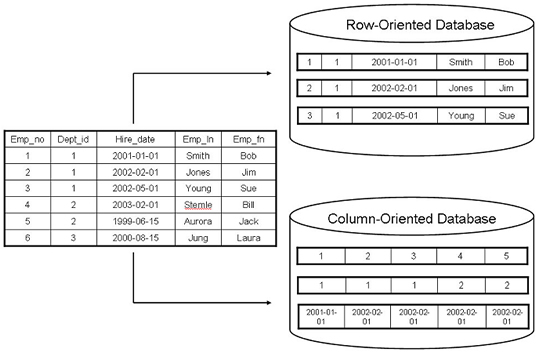
\includegraphics[width=0.7\linewidth]{column-oriented-database1.jpg}
  \caption{Row-based v/s Column-based data bases}
  \vspace{-0.2cm}
  \label{fig:blockdiagram}
  \vspace{-0.2cm}
\end{figure}

\end{itemize}

\section{Seek latency v/s Rotational latency}

\begin{itemize}
\item Seek latency defines the amount of time it takes a hard drive’s  read/write head to find the physical location of a piece of data on the  disk. 

\item Rotational latency is the delay waiting for the rotation of the disk to bring the required disk sector under the read-write head.

To reduce seek latency, temporal locality should be exploited. In general, seek latency is way higher than rotational latency.

\end{itemize}
\begin{figure}[ht]
  \centering
  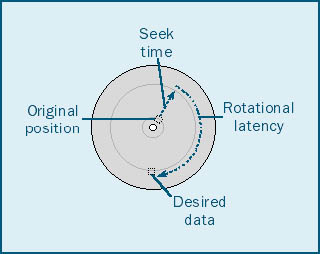
\includegraphics[width=0.7\linewidth]{seek_latency.jpg}
  \caption{Seek latency v/s Rotational latency}
  \vspace{-0.2cm}
  \label{fig:seek/rotational}
  \vspace{-0.2cm}
\end{figure}

\section{Disk Fragmentation}

Part of the files in a disk are distributed/spread across the disk (Non contiguous memory). This mechanism is referred to Disk fragmentation.

\section{Memory aligned loads and stores}

In aligned loads/stores, when a variable/address is loaded or stored the memory address must be a multiple of power of 2 bytes for example 8 or 16 etc. Now, if a variable/address is 13 bytes, and assume that each memory block/chunk is of  size - 4 bytes, then the respective variable takes 4 blocks and in the process 3 bytes are wasted and not used for other memory allocations.

\section{Internal fragmentation and External fragmentation}

\begin{itemize}
\item Internal fragmentation : In the previous example, (variable of 13 bytes taking 4 blocks, each block of 4 bytes) 3 bytes are wasted, in this scenario, the unusable memory is within an allocated region. This inefficient usage of memory is referred to {\bf internal fragmentation}

\item External fragmentation: Total memory space is enough to allocate memory for a requested variable, but the available memory is not contiguous because of this memory allocation cannot be completed. This is referred to {\bf external fragmentation}

\item Compaction saves/extract the free spaces between aligned memory allocation. This feature is available in Java(JVM) and is because of its garbage collection, which collects the unused memory periodically.

\end{itemize}

\section{Metadata overhead(book keeping) in Linux}

In Linux, initial bits of a memory allocation for a pointer stores the size of the pointer/variable(metadata of the pointer). This metadata is the overhead incurred in linux for storing the pointer.

\section{Memory allocation in Java v/s C/C++}

\begin{itemize}
\item In Java, memory for a object is allocated in scattered manner. For example, if a object A has 4 int variables, when instance of object A is allocated 4 variables are stored in non contiguous memory. This results in non temporal locality, and  inefficient pointer access. 

Note, in Java every object has a lock. 

\it In C++, variables of a class object are allocated in contiguous fashion, this results in better temporal locality, direct pointer access and control of object layout is possible.

\end{itemize}

\section{MapReduce v/s Hadoop}

\begin{itemize}
\item MapReduce is built on GFS file system and is implemented in C++, which translates to better performance compared to Hadoop. MapReduce is a closed source system and is developed by Google.

\item Hadoop is built on HDFS file system and is implemented in Java. It is a open source system and is developed by Yahoo!.

\end{itemize}

Java is not as efficient as C++, when performance is concerned as object layout can be controlled in C++ for faster object access and garbage collection of java constraints the performance. 

\section{Garbage collection in Java}

\begin{figure}[ht]
  \centering
  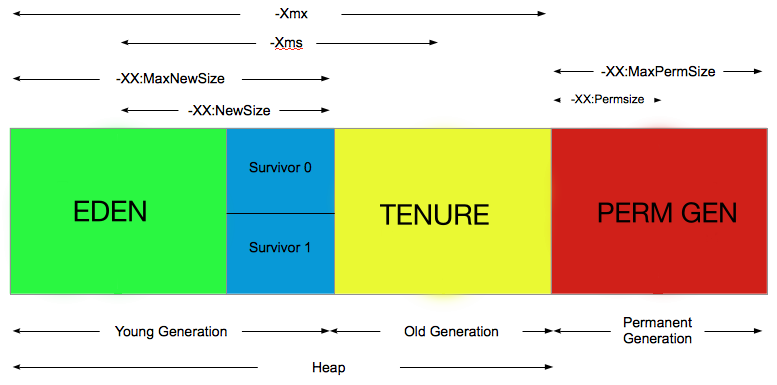
\includegraphics[width=0.7\linewidth]{jvm_heap.png}
  \caption{JVM Heap}
  \vspace{-0.2cm}
  \label{fig:jvm_heap}
  \vspace{-0.2cm}
\end{figure}

Young generation: Most of the newly created objects are located here. Since most objects soon become unreachable, many objects are created in the young generation, then disappear. 

Old generation: The objects that did not become unreachable and survived from the young generation are copied here. It is generally larger than the young generation. As it is bigger in size, the GC occurs less frequently than in the young generation. 

Garbage collection Tuning: The purpose of GC tuning is to minimize the number of objects passed to the old area and to decrease Full GC execution time. GC tuning is required for the optimized application performance, as GC can take up high CPU resources which increases the running times of the applications.

\end{document}
